\chapter{Identifying and Classifying Emission-line Spectra: The End-to-end Pipeline}

\section{Drawing Conclusions from Prior Chapters}

The following conclusions can be drawn from the results presented in the preceding chapters:

\begin{enumerate}
    \item The curse of dimensionality presents a significant challenge when working with high-resolution data from million star surveys such as GALAH DR3. 
    \item Dimensionality reduction methods such as t-SNE may not be sufficiently robust at identifying emission-line spectra. Furthermore, the two dimensional t-SNE representation may not be sensitive to the morphological differences between emission-line spectra and non-emission line spectra.
    \item Given a data set with emission-line spectra, DTW-based agglomerative hierarchical clustering can be used effectively to identify and categorise P Cygni, inverse P Cygni and other emission-line spectra.
\end{enumerate}

This chapter builds on these conclusions and presents a proof of concept pipeline for the identification and classification of emission-line spectra. DTW-based agglomerative hierarchical clustering, which  was introduced in Chapter 4, forms the basis of this pipeline. Furthermore, this pipeline relies on the pre-selection of H$\alpha$ emission-line spectra using an autoencoder first introduced by \citet{vcotar2021galah}. In this chapter, the full GALAH DR3 data set will be utilised, as opposed to the much smaller H$\alpha$ emission-line star data set provided by \citet{vcotar2021galah}, which was used extensively in Chapter 4 and Chapter 5.

\section{Identifying H$\alpha$ Emission-line Spectra}

Chapter 2 presented an autoencoder neural network developed by \citet{vcotar2021galah} that is capable of identifying H$\alpha$ emission-line spectra. This method was adapted as a pre-processing step prior to the application of the DTW-based agglomerative hierarchical clustering technique demonstrated in Chapter 4. The autoencoder method is as follows:

The autoencoder learns the latent space representation of non-emission line spectra but \emph{does not} learn the latent space representation of emission-line spectra accurately. This latent space represents each higher dimensional high resolution spectrum as a five dimensional vector. This process is known as encoding. Once the training phase is completed, the autoencoder is fed the total DR3 data set to generate predictions for each spectrum. This process is known as decoding. 

The training data are deliberately biased towards non-emission line spectra (so-called normal or typical spectra). Thus the predicted spectra will match the data for non-emission-line spectra more accurately than for emission-line spectra. The flux difference between a predicted spectrum and its observed (original) data counterpart can be used to flag emission-line stars. This flagging can be accomplished by computing the equivalent width of this "difference spectrum" around the H$\alpha$ line.

\subsection{The Autoencoder Architecture and Training}

The autoencoder architecture presented here is similar to the work of \citet{vcotar2021galah} and maps high resolution spectra of dimension 4,459 to a five dimensional latent space. The popular deep-learning frameworks \texttt{tensorflow} \citep{tensorflow2015-whitepaper} and \texttt{keras} \citep{chollet2015keras} were used to develop the autoencoder.

Each successive dense layer in the neural network reduces the dimensionality of the input layer successively by 75\%, 50\%, 25\% and finally by 10\%. Each layer was activated by the non-linear PReLU function \citep{he2015delving}. The training loss is minimised using the Adam optimiser which performs gradient descent \citep{kingma2014adam}.

\begin{figure}[!htb]
\centering
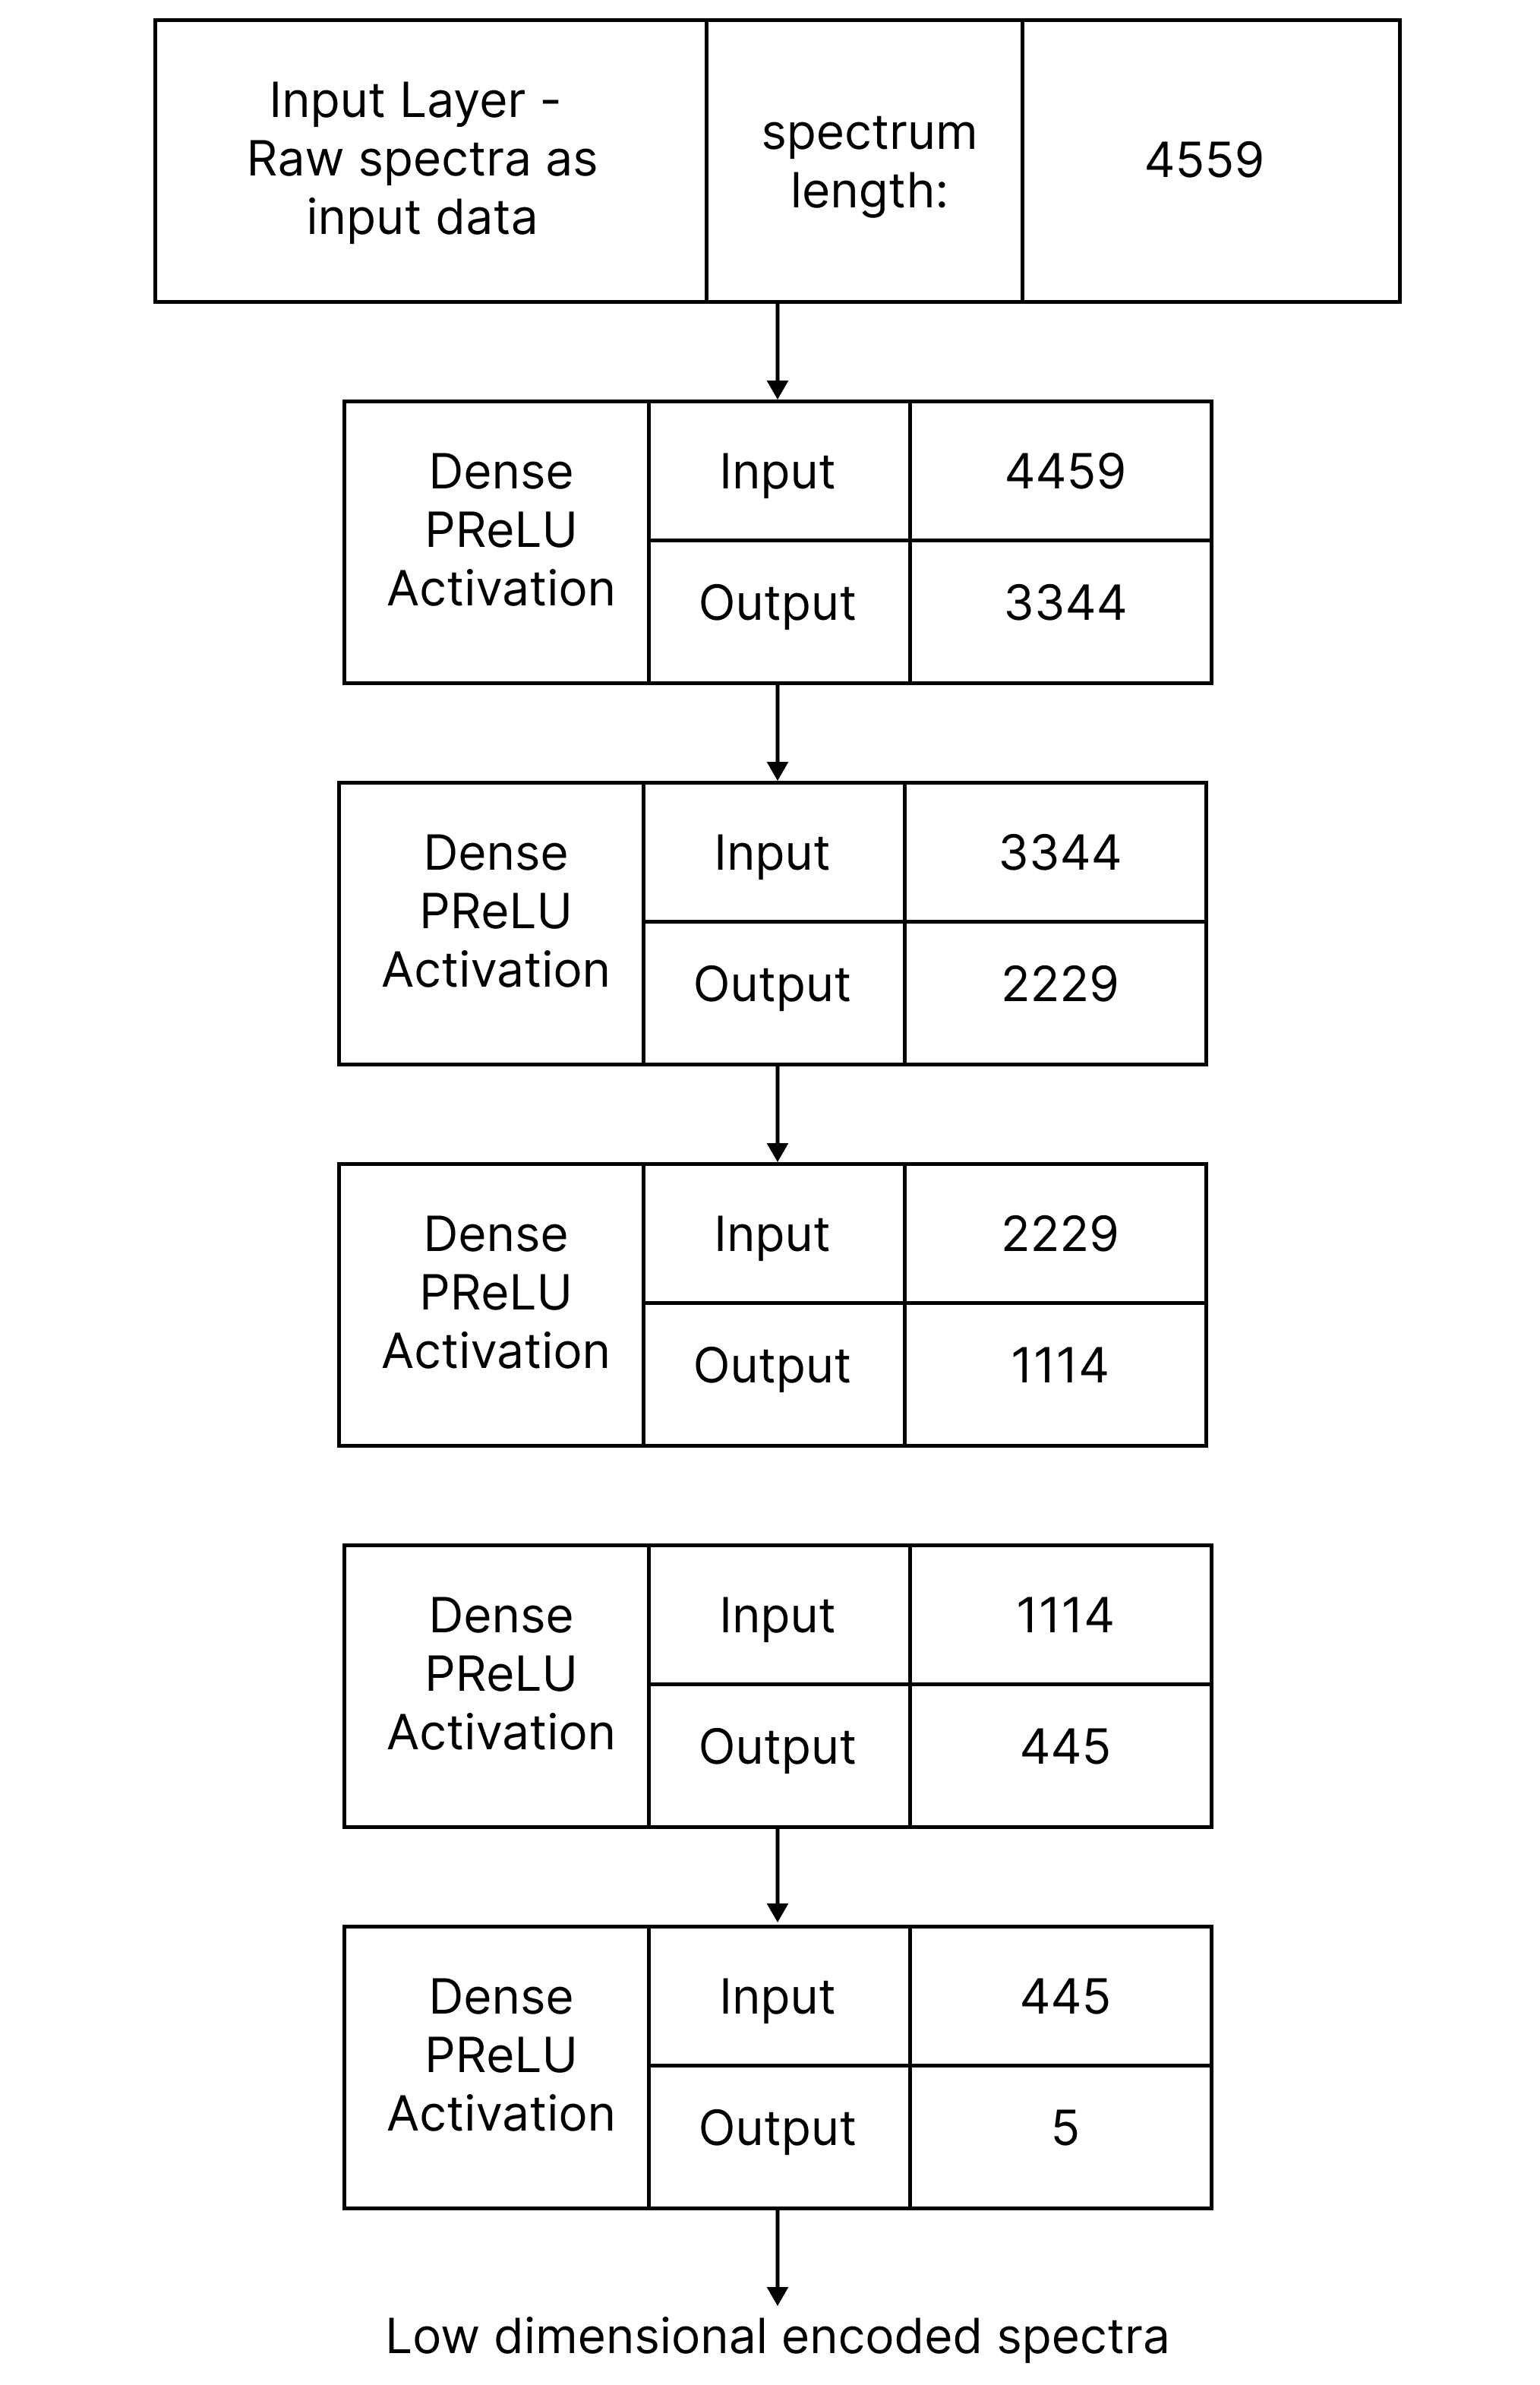
\includegraphics[scale=0.13]{figures/autoencoder diagram.png}
\caption{Visual representation of the encoder. The value in
the right most column of each layer indicates the number of input and output
connections to neighboring layers.}
\end{figure}

\citet{vcotar2021galah} recommended inverting the flux values (1 - normalised flux) prior to training and prediction. Greater training stability was achieved by this inversion. Furthermore, they recommended an epoch size of 350 and a batch size of 40,000 spectra. For validation, 10\% of the samples were selected and set aside. This work followed the same conventions. 

For training, the autoencoder required a training set that is either significantly biased towards non-emission line spectra around H$\alpha$, or better yet, contains exclusively non-emission-line spectra. In order to select these spectra in DR3, the quality criteria recommended by \citet{vcotar2021galah}, \citet{buder2021galah+} and \citet{kos2017galah} were applied. 

While these criteria may not fully guarantee that the autoencoder will be trained exclusively on non-emission line spectra, prior work by \citet{vcotar2021galah} indicated that the criteria are sufficiently robust for the purpose of training this specific network. The Data Central SQL/ADQL catalogue query service was used to retrieve GALAH DR3 \texttt{sobject\_id} values that matched these criteria—namely:

\begin{lstlisting}[language=SQL]
SELECT sobject_id
FROM   galah_dr3.main_star
WHERE  snr_c3_iraf > 30
       AND red_flag = 0
       AND flag_sp < 16 
\end{lstlisting}

\begin{table}[!htb]
\begin{center}
\begin{tabular}{|l|l|}
\hline
\textbf{Criterion}    & \textbf{Rationale}                                                                 \\ \hline
SNR \textgreater 30   & Spectra have reduced noise contamination      \\ \hline
\texttt{red\_flag} = 0         & Select spectra that have no know reduction issues                                  \\ \hline
\texttt{flag\_sp} \textless 16 & Select spectra that do not include known emission-line spectra identified by t-SNE \\ \hline
\end{tabular}
\caption{GALAH DR3 selection criteria for non-emission line spectra for training purposes.}
\label{table:Selection Criteria}
\end{center}
\end{table}
This query returned 396,338 spectra. The red arm data was re-sampled to a common wavelength grid using the method outlined in Chapter 3. The normalised flux was then inverted and used as the training data set.

\begin{figure}[!htb]
\centering
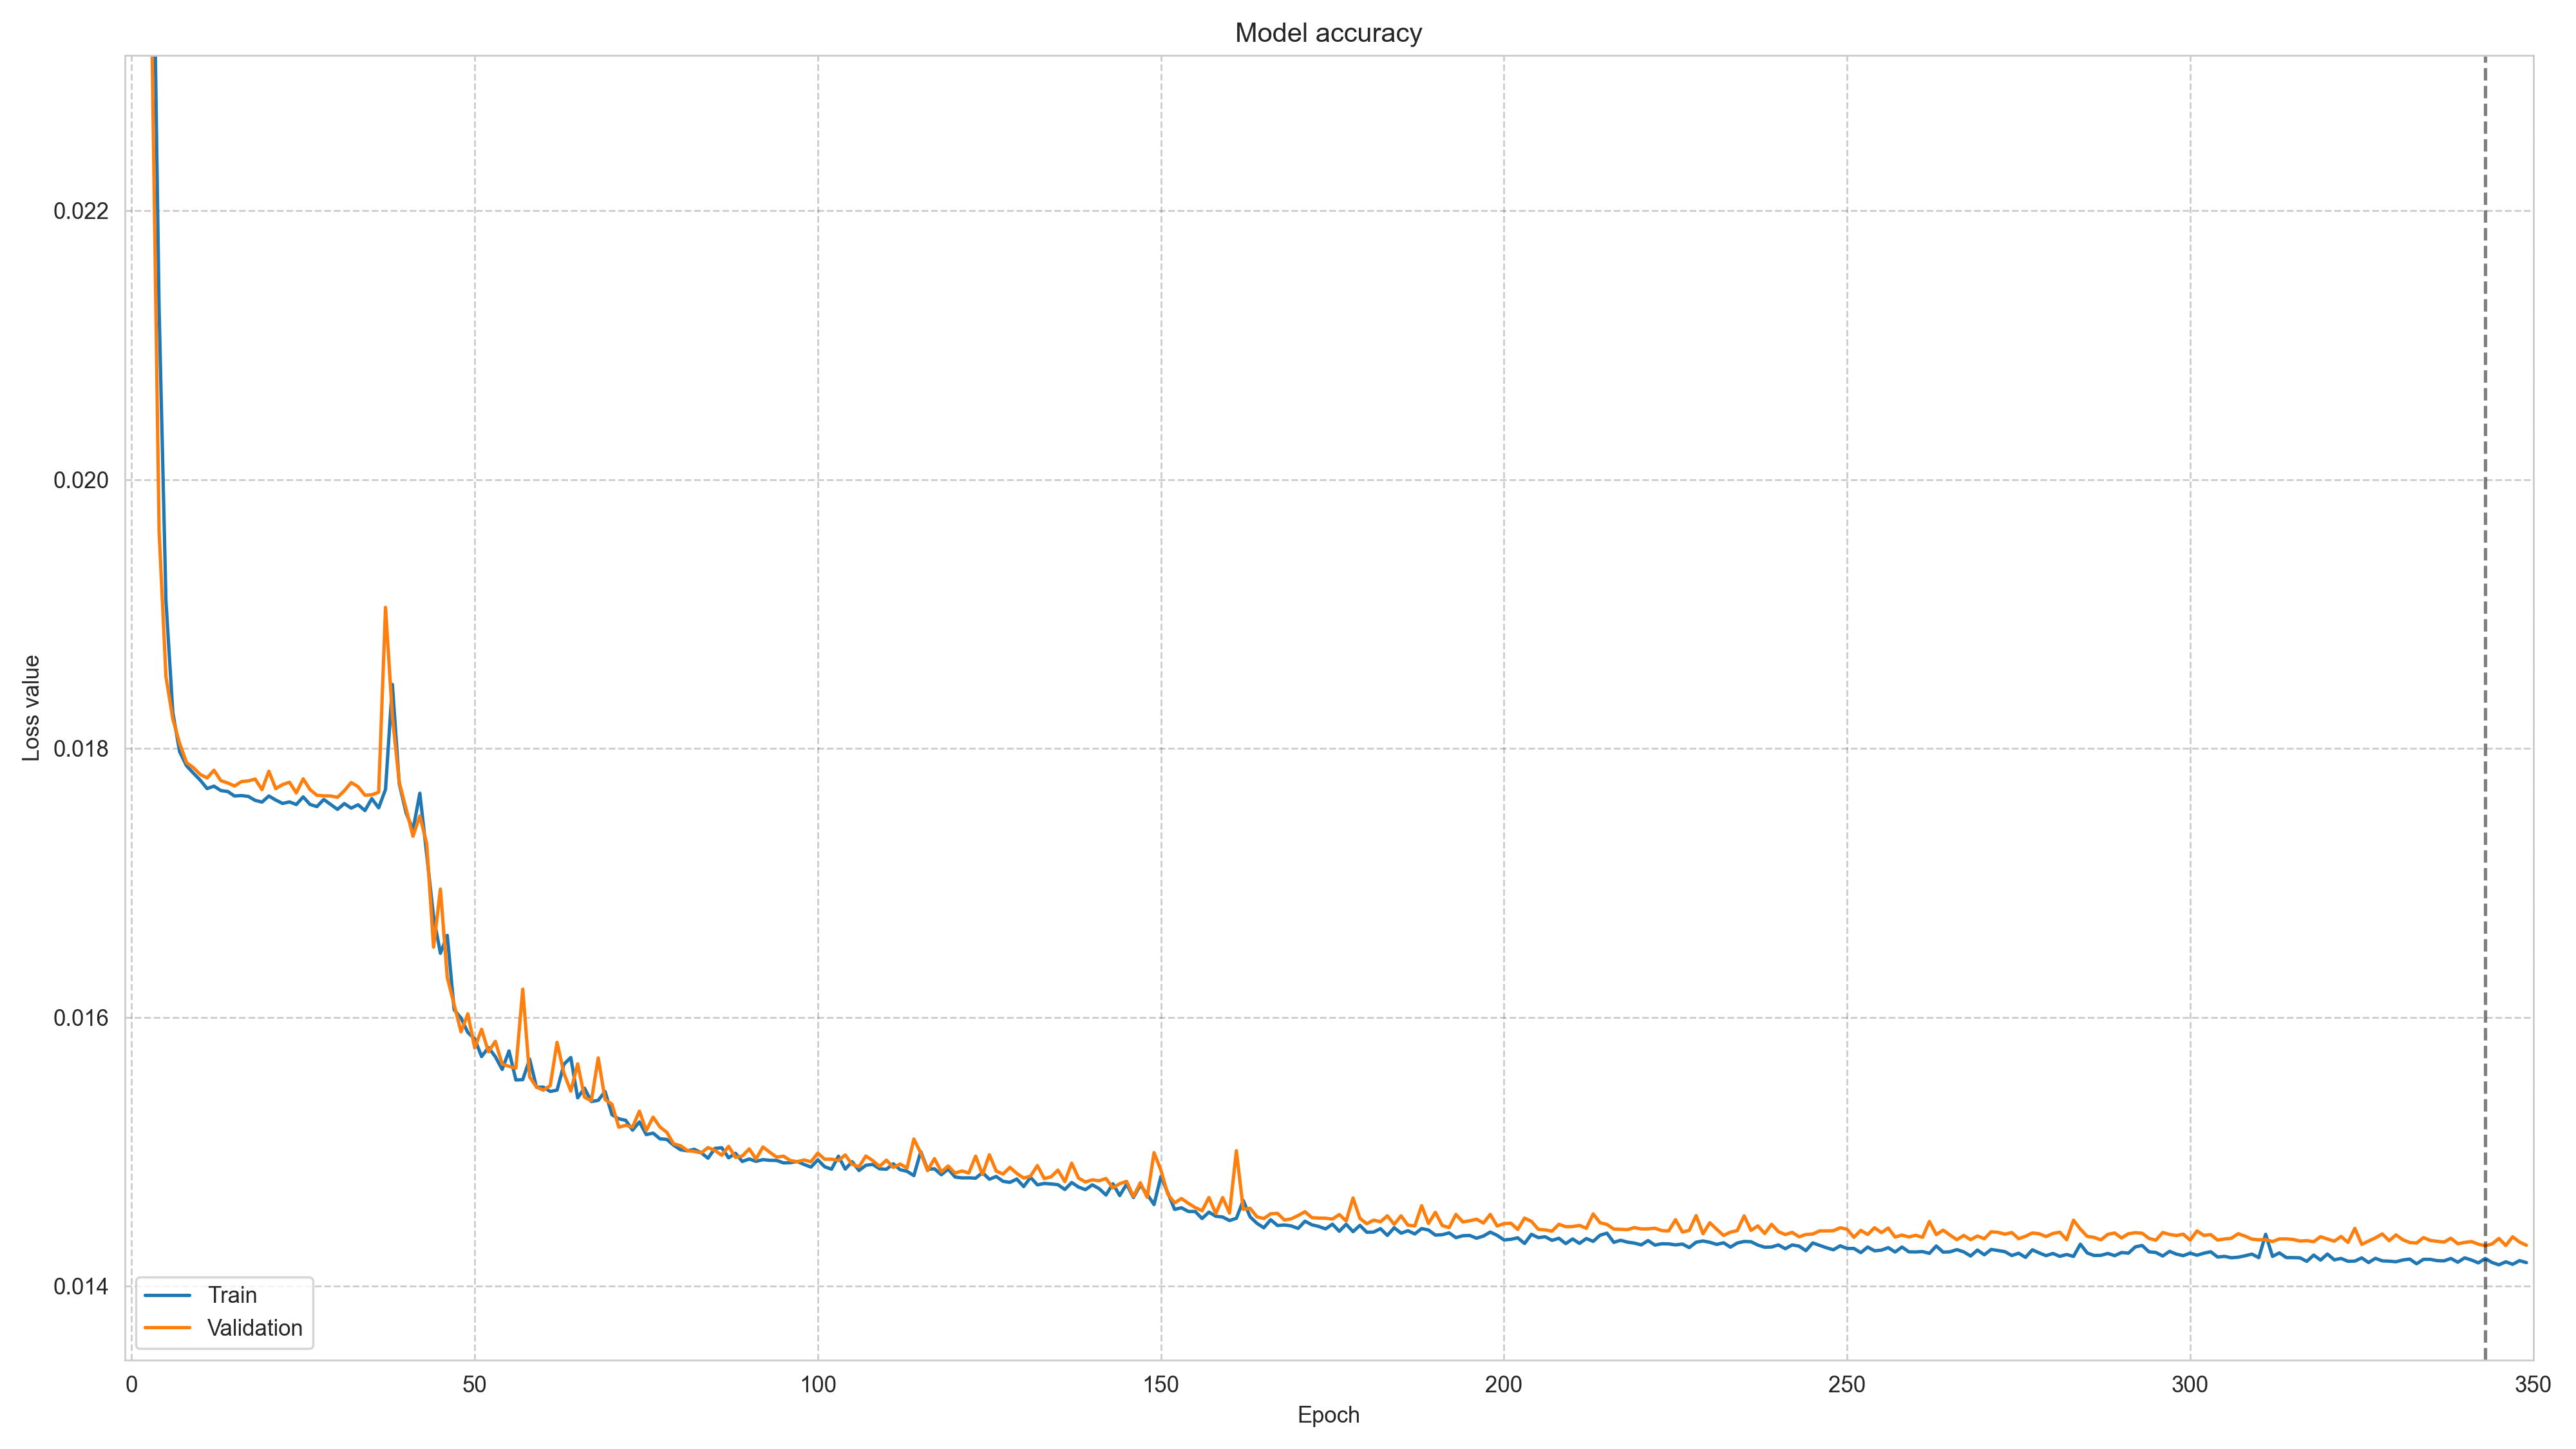
\includegraphics[scale=0.38]{figures/ann_network_loss.png}
\caption{Prediction accuracy of the red arm training data set at different training epochs.}
\label{fig6.2}
\end{figure}
The autoencoder was applied to these data and the prediction error for training was computed as a sum of all absolute differences between the input and output data sets. The results are presented in Figure \ref{fig6.2}, which shows the prediction error as a function of epoch. These results are quite comparable to those presented in \citet{vcotar2021galah}.

It is expected that the autoencoder will perform poorly when attempting to reconstruct or predict emission-line spectra/fluxes. Conversely, it is expected that it will perform well on emission-line spectra. This behaviour has significant implications for the detection of H$\alpha$ emission-line spectra. This is discussed in the next section.

\subsection{Using Difference Spectra to Identify Emission-line Spectra}

Once the autoencoder was trained, data from GALAH DR3 were fed to the network. The network decoded these spectra and provided predictions for each spectrum based on the latent space representation it had learned. Since the input data during the training phase were inverted, for consistency of operation all DR3 spectra were inverted prior to being fed into the network. Predicted results from the autoencoder were also inverted.

The difference spectra between the predicted and the original DR3 spectra (observed spectra) were computed using Formula \ref{formula:6.1}. Presented below are the inverted difference spectra for a known non-emission line spectrum (Figure \ref{fig6.3}) and a known emission-line spectrum (Figure \ref{fig6.4}) in DR3 around H$\alpha$. The emission-line spectrum, which is a P Cygni, was identified from the work presented in Chapter 4. Note that the non-emission-line spectrum produces a difference spectrum with an approximately flat response, while the emission-line spectrum does not. 

\begin{equation}
   f_{difference} = f_{observed} - f_{predicted}
\label{formula:6.1}
\end{equation}

\begin{figure}[!htb]
\centering
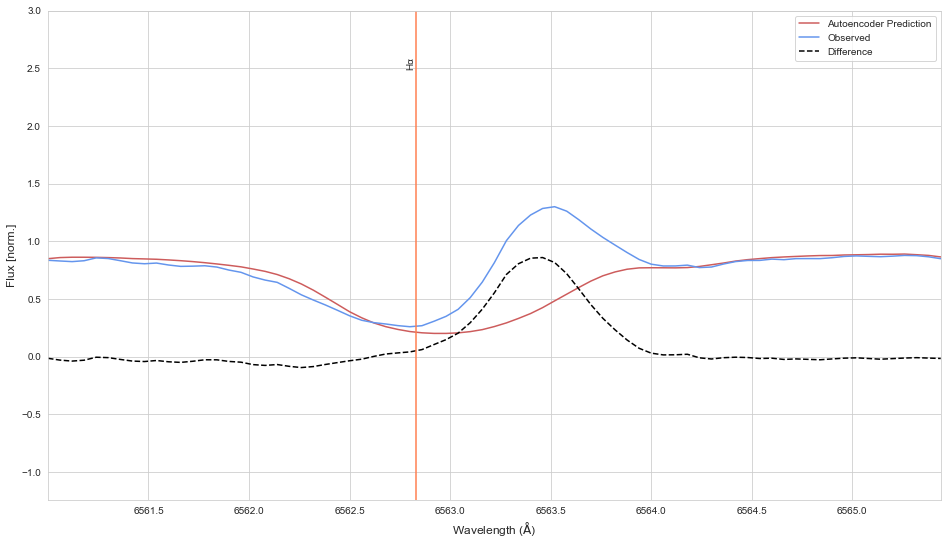
\includegraphics[scale=0.45]{figures/normal difference.png}
\caption{An emission-line spectrum (P Cygni), the autoencoder prediction and corresponding difference spectrum. Note the non-flat response of the difference spectrum. This response can be quantified by calculating its equivalent width.}
\label{fig6.3}
\end{figure}

\begin{figure}[!htb]
\centering
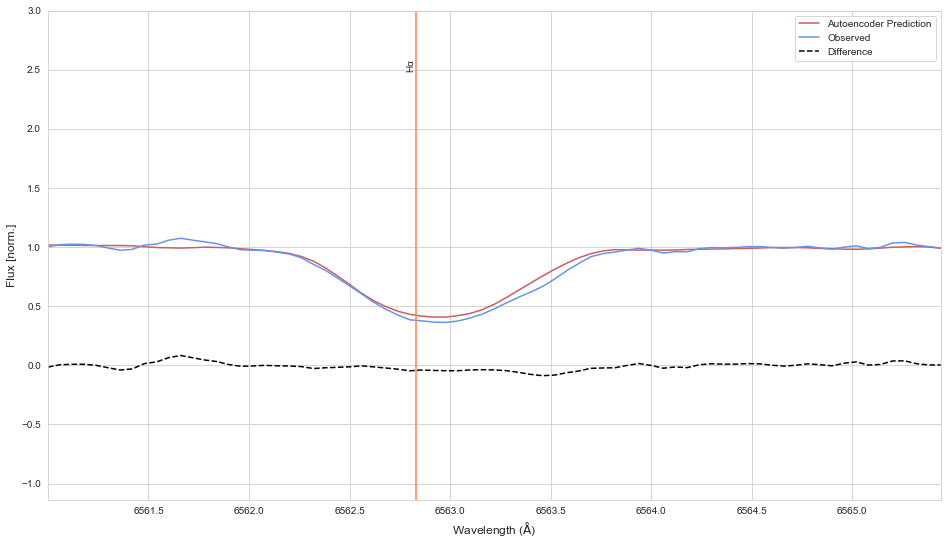
\includegraphics[scale=0.45]{figures/non emission difference.png}
\caption{A non-emission-line spectrum, the autoencoder prediction and corresponding difference spectrum. Note the flat response of the difference spectrum. This response can be quantified by calculating its equivalent width.}
\label{fig6.4}
\end{figure}

The equivalent width within the range 6561\r{A} - 6565\r{A} was determined using the popular Python packages \texttt{astropy} \citep{astropy:2018, astropy:2013} and \texttt{specutils} \citep{specutils}. For consistency, these widths were calculated for the inverted difference spectra. \citet{vcotar2021galah} used an equivalent width cut-off of 0.25 to separate emission-line spectra from DR3. The sensitivity of this cut-off parameter was tested. Selecting a lower threshold for this parameter, such as EW > 0.20,  allows for a wider selection of potential H$\alpha$ emission-line spectra, while a higher threshold such as EW > 0.50 may restrict the selection to only the strongest emitters. The rationale for choosing EW > 0.25 in \citet{vcotar2021galah} was presumably based on a trial and error approach. A similar empirical strategy to fine-tune this parameter and select a reasonable population of H$\alpha$ emission-line spectra resulted in setting EW > 0.22. This value provided the best overall performance. However, this cut-off does not guarantee that the maximum number of H$\alpha$ emission-line spectra was selected. 

Given that \citet{vcotar2021galah} used a different population for their work, the H$\alpha$ emission-line spectra discovered cannot be directly compared to those found in GALAH DR3 using the method above. It can be noted that, due to the inclusion of data from other surveys, only 4,556 out of 10,364 objects identified by \citet{vcotar2021galah} were present in the GALAH DR3 sample, which comprised 396,338 spectra. These 4,556 were also captured and recovered within the H$\alpha$ emission-line spectra discovered using the autoencoder and setting EW > 0.22. The summary statistics for each sample are provided in the Appendix.

\begin{figure}[!htb]
\centering
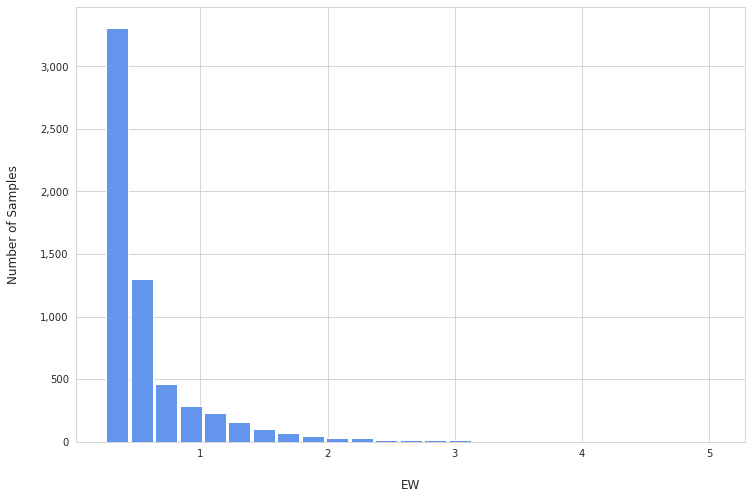
\includegraphics[scale=0.50]{figures/EW hist.png}
\caption{The equivalent width (EW) distribution of the inverted difference spectra of the emission-line spectra identified in GALAH DR3. Here EW > 0.22.}
\end{figure}


\section{Applying Dynamic Time Warping and Agglomerative Hierarchical Clustering}

Once the H$\alpha$ emission-line spectra were selected, the data were passed to the next step of the analytics pipeline. The DTW distance matrix was computed for each spectrum, ensuring that only masked data were presented to the \texttt{FastDTW} algorithm \citep[the masked region being 6561\r{A} - 6565\r{A};][]{traven2017galah}. As mentioned in Chapter 4, this approach significantly reduces run-time and computational complexity. 

\begin{figure}[!htb]
\centering
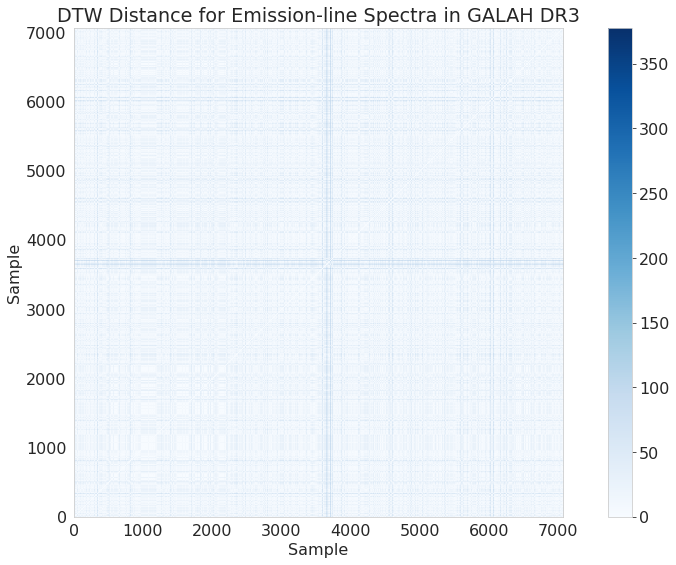
\includegraphics[scale=0.50]{figures/dtw distances dr3.png}
\caption{Pairwise DTW distances for emission line spectra identified in DR3. Darker colours indicate samples that are dissimilar.}
\end{figure}

\begin{figure}[!htb]
\centering
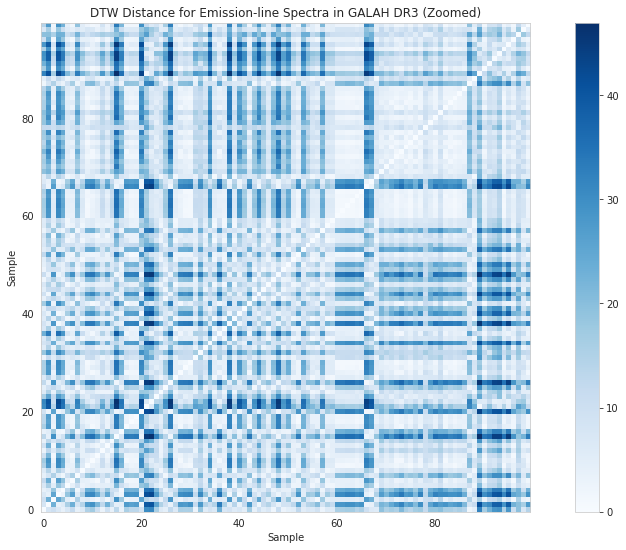
\includegraphics[scale=0.50]{figures/dtw distances dr3 zoomed.png}
\caption{Pairwise DTW distances for emission line spectra identified in DR3 (zoomed). Darker colours indicate samples that are dissimilar.}
\end{figure}

Once the distance calculation was completed, agglomerative hierarchical clustering was performed ensuring complete linkage. At this stage, this work deviated from the number of clusters used in Chapter 4; for one thing, many of the H$\alpha$ emission-line spectra identified in the previous stage of the pipeline exhibited noticeably more complex emission-line morphologies than those identified by \citet{vcotar2021galah}. 

This richer variety of morphologies can be attributed to the fact that the DR3 population is fundamentally different to the survey data used by \citet{vcotar2021galah} This can be demonstrated by observing the number of P Cygni spectra that separate into a cluster as the number of clusters is increased beyond the value (10) used in Chapter 4; with H$\alpha$ emission-line stars identified in the DR3 dataset, the maximum number of P Cygni and inverse P Cygni were separated when the number of clusters was set to 45. This is significantly higher than what was observed in the results presented in Chapter 4. The tree generated by agglomerative hierarchical clustering is thus cut at a depth of 45 (as opposed to 10) for this specific sample for a maximal separation of P Cygni and inverse P Cygni spectra. 

\begin{figure}[!htb]
\centering
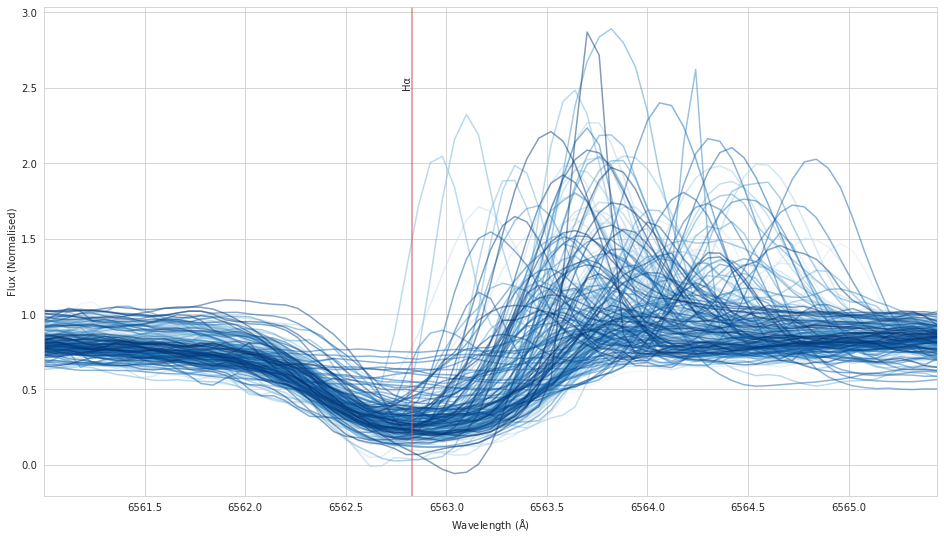
\includegraphics[scale=0.45]{figures/p cygni ensemble.png}
\caption{Ensemble plot of 243 P Cygni spectra identified in DR3 using DTW.}
\end{figure}

\begin{figure}[!htb]
\centering
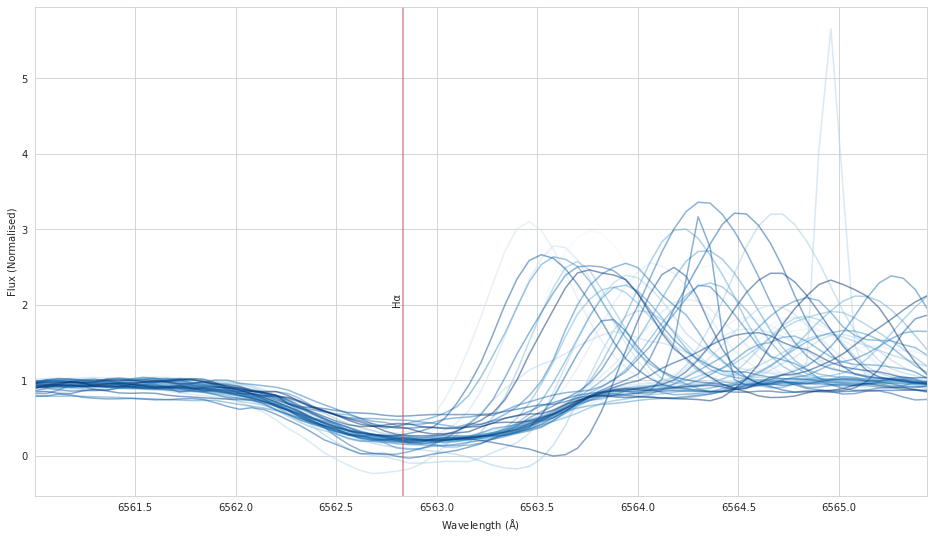
\includegraphics[scale=0.45]{figures/p cugni 2.png}
\caption{Ensemble plot of 53 additional P Cygni spectra identified in DR3 using DTW. These were not included in the main P Cygni cluster but appeared in a separate group, likely due to a less prominent absorption feature blueward of H$\alpha$}.
\end{figure}

\begin{figure}[!htb]
\centering
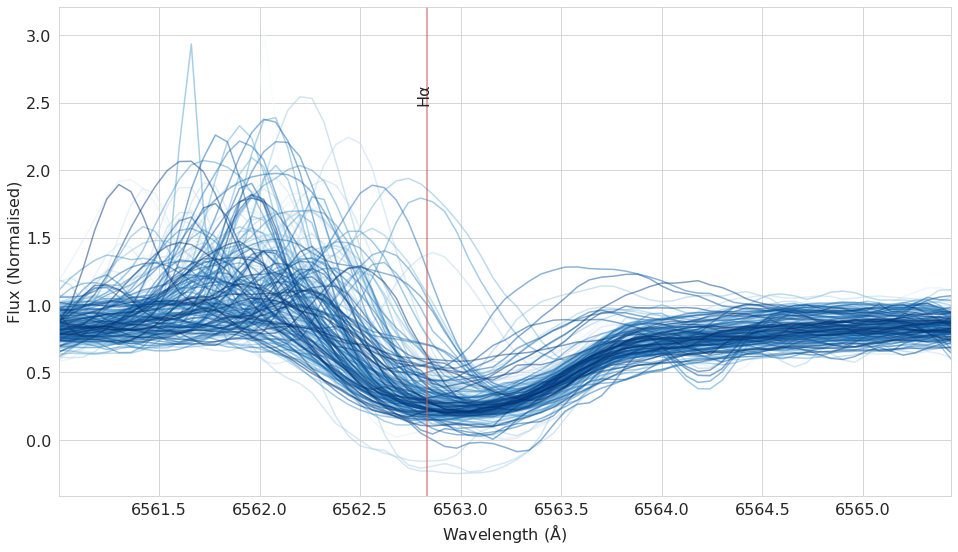
\includegraphics[scale=0.45]{figures/inverse p cygni ensemble.png}
\caption{Ensemble plot of 219 inverse P Cygni spectra identified in DR3 using DTW.}
\end{figure}

The significant advantage of utilizing a higher number of clusters than 10 is that if, as in the case of DR3, more peculiar emission-line spectra are present, they will be separated from the total data set more effectively, i.e., there is no scheme by which these extremely peculiar yet rare spectra can hide in a larger set of data points. These peculiar spectra would form their own minority clusters within the overall hierarchy of the tree generated by the clustering procedure. As far as the author is aware, there exists no precedent in literature for selecting 45 distinct classes for emission-line spectra. However, given that the process outlined here is entirely data driven, it is justifiable, since this value creates maximal separation of P Cygni and inverse P Cygni spectra, as well as the separation of peculiar sub-species in DR3 which have not been classified previously. Additional details of these are provided in the Appendix. Further inspection of key classes were carried out using an interactive plotting tool created by using the \texttt{plotly} package.

\begin{figure}[!htb]
\centering
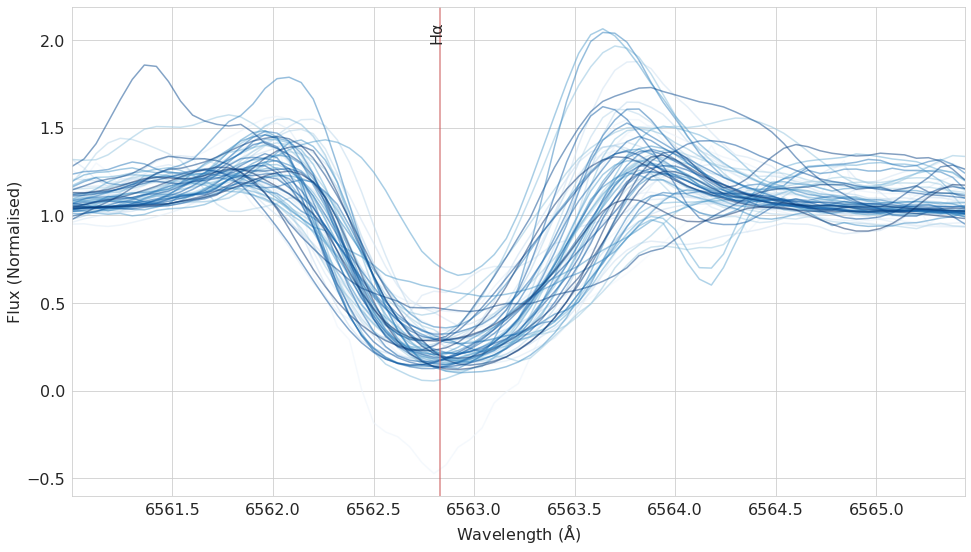
\includegraphics[scale=0.45]{figures/double peak 1.png}
\caption{Ensemble plot of 67 double peaked emission-line spectra identified in DR3 using DTW.}
\end{figure}

\begin{figure}[!htb]
\centering
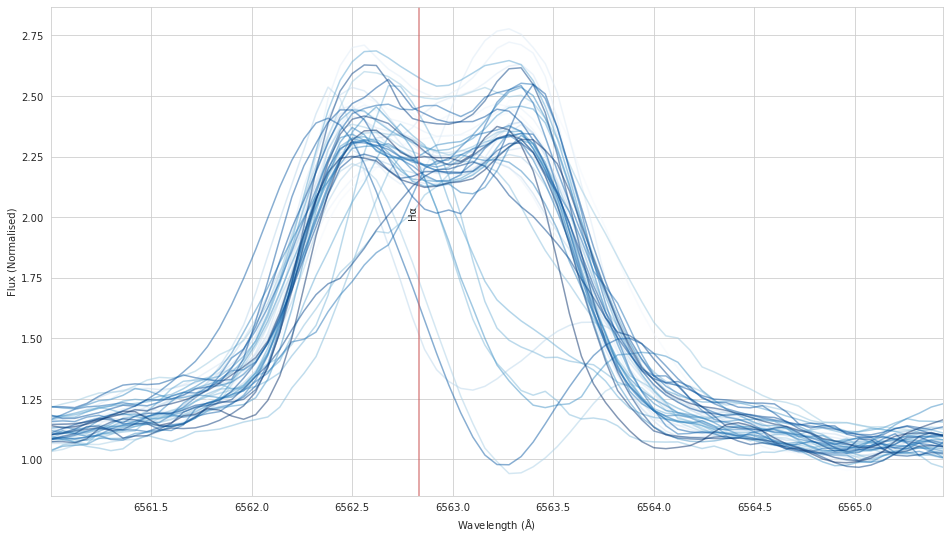
\includegraphics[scale=0.45]{figures/emission on abs.png}
\caption{Ensemble plot of 46 self-absorption type spectra identified in DR3 using DTW.}
\end{figure}

\begin{figure}[!htb]
\centering
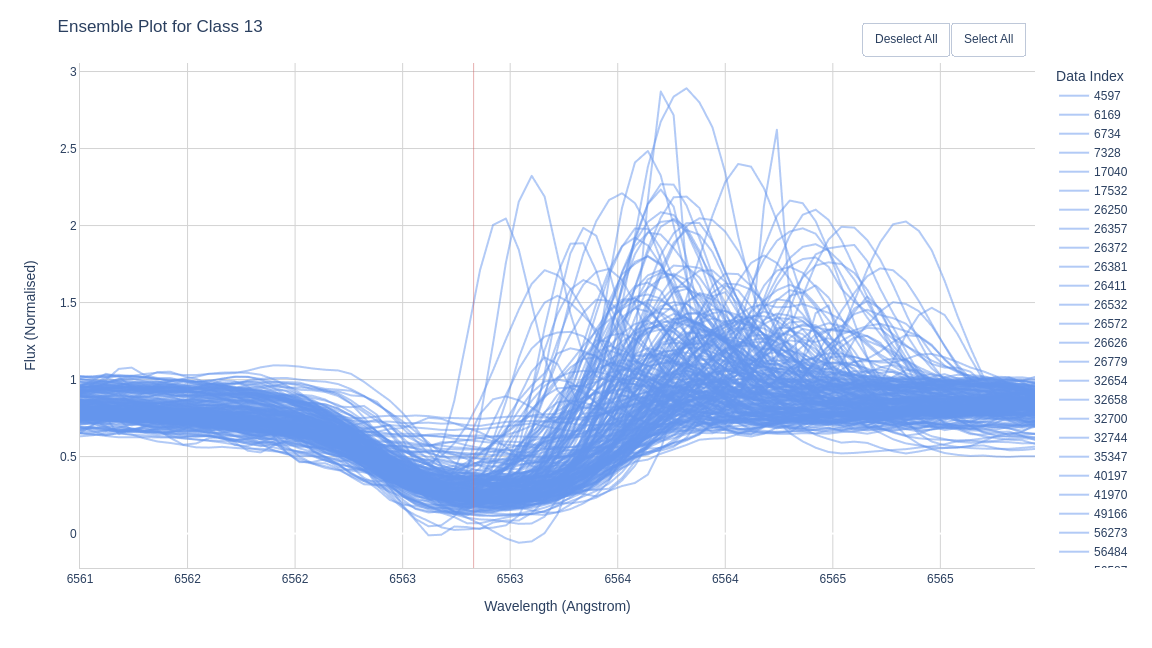
\includegraphics[scale=0.38]{figures/plotly image.png}
\caption{Inspecting a class of spectra identified by DTW using a \texttt{plotly} plot which changes interactively based on the object selected.}
\end{figure}

\section{Concluding Remarks}

Identifying atypical spectra such as emission-line spectra from a data set that contains a majority of typical spectra is a challenging task for machine learning methods. After analysing the requirement and end goals, a unique and powerful combination of methods such as dimensionality reduction, anomaly detection using autoencoders and dynamic time warping was  carefully selected to identify and cluster emission-line spectra in the GALAH DR3 dataset. 

Apart from selecting the number of clusters, the pipeline presented in this work requires significantly less human intervention than other methods in literature. Crucially, it does not require human intervention to manually identify emission-line spectra from a large data set such as GALAH DR3. 

Using these methods, this work was able to identify 296 P Cygni spectra and 219 inverse P Cygni spectra, as well as numerous other classes of stars with H$\alpha$ emission. This leads to the conclusion that, in instances where atypical spectra are hidden in a data set which comprises a majority of typical spectra, this novel approach is able to outperform the machine learning methods presented to date in the literature. 







